\documentclass[a3paper,landscape]{article}
\usepackage[margin=1.5cm]{geometry}
\usepackage[utf8]{inputenc}
\usepackage[T1]{fontenc}
\usepackage{tikz}
\usetikzlibrary{positioning,arrows.meta,shapes.geometric,fit,backgrounds}
\usepackage[table]{xcolor}
\usepackage{amsmath,amssymb}
\usepackage{parskip}
\usepackage{microtype}
\pagestyle{empty}

\begin{document}

\begin{center}
{\Large\bfseries Electrochemical Wound Biosensor: Modelling Pipeline}\\[0.5em]
{\normalsize Eton iGEM 2026 \quad|\quad MMP-9 / HNE Ratiometric SWV Sensor}\\[0.3em]
\end{center}

\vspace{0.6em}

\begin{center}
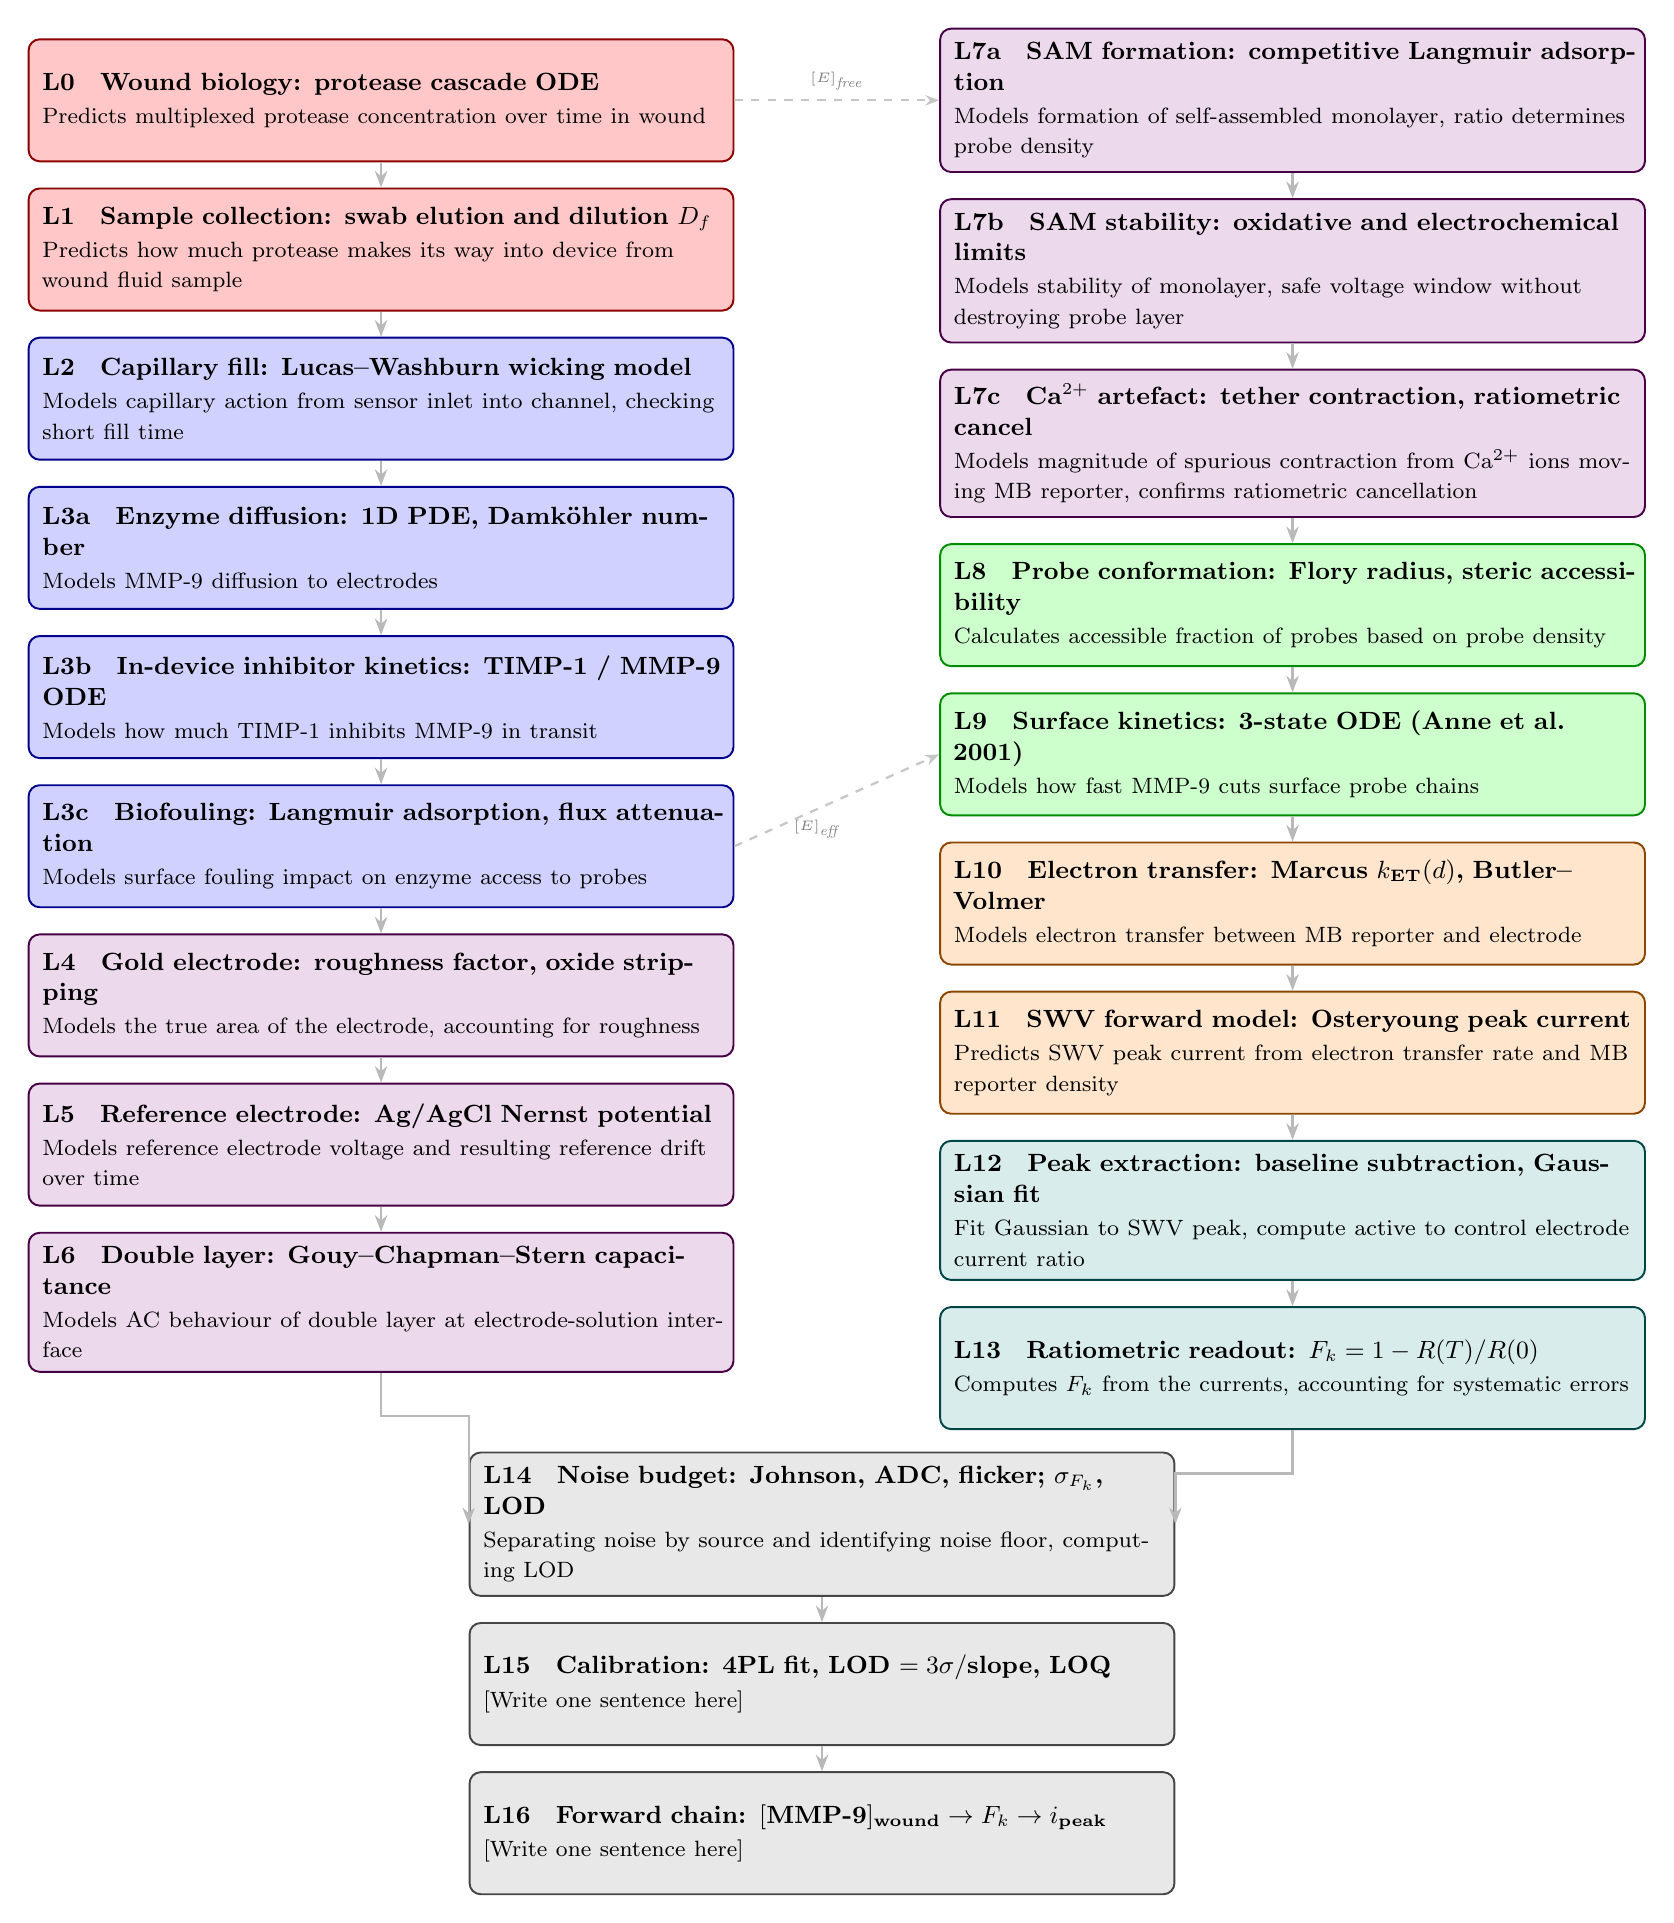
\begin{tikzpicture}[
  node distance=0.32cm and 1.6cm,
  lbox/.style={
    rectangle, rounded corners=4pt,
    minimum width=8.8cm, minimum height=1.55cm,
    text width=8.6cm, align=left,
    font=\small, inner sep=5pt
  },
  singlearr/.style={-{Stealth[length=6pt]}, thick, draw=gray!55},
  dasharr/.style={-{Stealth[length=5pt]}, dashed, draw=gray!45, thick},
  bio/.style  ={lbox, fill=red!22,    draw=red!55!black,    line width=0.7pt},
  trans/.style={lbox, fill=blue!18,   draw=blue!55!black,   line width=0.7pt},
  elec/.style ={lbox, fill=violet!15, draw=violet!55!black, line width=0.7pt},
  kin/.style  ={lbox, fill=green!20,  draw=green!55!black,  line width=0.7pt},
  swv/.style  ={lbox, fill=orange!20, draw=orange!55!black, line width=0.7pt},
  sig/.style  ={lbox, fill=teal!15,   draw=teal!55!black,   line width=0.7pt},
  cal/.style  ={lbox, fill=gray!18,   draw=gray!55!black,   line width=0.7pt},
  layerlabel/.style={font=\bfseries\small},
  desc/.style={font=\footnotesize\itshape, text=gray!70!black},
]

%% ── LEFT COLUMN (L0 – L8) ─────────────────────────────────────────────────

\node[bio] (L0) {
  \textbf{L0 \; Wound biology: protease cascade ODE}\\[1pt]
  \footnotesize
  Predicts multiplexed protease concentration over time in wound
};

\node[bio,   below=of L0]  (L1) {
  \textbf{L1 \; Sample collection: swab elution and dilution $D_f$}\\[1pt]
  \footnotesize
  Predicts how much protease makes its way into device from wound fluid sample
};

\node[trans, below=of L1]  (L2) {
  \textbf{L2 \; Capillary fill: Lucas--Washburn wicking model}\\[1pt]
  \footnotesize
  Models capillary action from sensor inlet into channel, checking short fill time
};

\node[trans, below=of L2]  (L3a) {
  \textbf{L3a \; Enzyme diffusion: 1D PDE, Damk\"{o}hler number}\\[1pt]
  \footnotesize
  Models MMP-9 diffusion to electrodes
};

\node[trans, below=of L3a] (L3b) {
  \textbf{L3b \; In-device inhibitor kinetics: TIMP-1 / MMP-9 ODE}\\[1pt]
  \footnotesize
  Models how much TIMP-1 inhibits MMP-9 in transit
};

\node[trans, below=of L3b] (L3c) {
  \textbf{L3c \; Biofouling: Langmuir adsorption, flux attenuation}\\[1pt]
  \footnotesize
  Models surface fouling impact on enzyme access to probes
};

\node[elec,  below=of L3c] (L4) {
  \textbf{L4 \; Gold electrode: roughness factor, oxide stripping}\\[1pt]
  \footnotesize
  Models the true area of the electrode, accounting for roughness
};

\node[elec,  below=of L4]  (L5) {
  \textbf{L5 \; Reference electrode: Ag/AgCl Nernst potential}\\[1pt]
  \footnotesize
  Models reference electrode voltage and resulting reference drift over time
};

\node[elec,  below=of L5]  (L6) {
  \textbf{L6 \; Double layer: Gouy--Chapman--Stern capacitance}\\[1pt]
  \footnotesize
  Models AC behaviour of double layer at electrode-solution interface
};

%% ── RIGHT COLUMN (L7a – L13) ─────────────────────────────────────────────

\node[elec,  right=2.6cm of L0]  (L7a) {
  \textbf{L7a \; SAM formation: competitive Langmuir adsorption}\\[1pt]
  \footnotesize
  Models formation of self-assembled monolayer, ratio determines probe density
};

\node[elec,  below=of L7a] (L7b) {
  \textbf{L7b \; SAM stability: oxidative and electrochemical limits}\\[1pt]
  \footnotesize
  Models stability of monolayer, safe voltage window without destroying probe layer
};

\node[elec,  below=of L7b] (L7c) {
  \textbf{L7c \; Ca$^{2+}$ artefact: tether contraction, ratiometric cancel}\\[1pt]
  \footnotesize
  Models magnitude of spurious contraction from Ca$^{2+}$ ions moving MB reporter, confirms ratiometric cancellation
};

\node[kin,   below=of L7c] (L8) {
  \textbf{L8 \; Probe conformation: Flory radius, steric accessibility}\\[1pt]
  \footnotesize
  Calculates accessible fraction of probes based on probe density
};

\node[kin,   below=of L8]  (L9) {
  \textbf{L9 \; Surface kinetics: 3-state ODE (Anne et al.\ 2001)}\\[1pt]
  \footnotesize
  Models how fast MMP-9 cuts surface probe chains
};

\node[swv,   below=of L9]  (L10) {
  \textbf{L10 \; Electron transfer: Marcus $k_\text{ET}(d)$, Butler--Volmer}\\[1pt]
  \footnotesize
  Models electron transfer between MB reporter and electrode
};

\node[swv,   below=of L10] (L11) {
  \textbf{L11 \; SWV forward model: Osteryoung peak current}\\[1pt]
  \footnotesize
  Predicts SWV peak current from electron transfer rate and MB reporter density
};

\node[sig,   below=of L11] (L12) {
  \textbf{L12 \; Peak extraction: baseline subtraction, Gaussian fit}\\[1pt]
  \footnotesize
  Fit Gaussian to SWV peak, compute active to control electrode current ratio
};

\node[sig,   below=of L12] (L13) {
  \textbf{L13 \; Ratiometric readout: $F_k = 1 - R(T)/R(0)$}\\[1pt]
  \footnotesize
  Computes $F_k$ from the currents, accounting for systematic errors
};

%% ── BOTTOM ROW (L14 – L16) ───────────────────────────────────────────────

\node[cal, below=1.0cm of L6,  xshift=5.6cm] (L14) {
  \textbf{L14 \; Noise budget: Johnson, ADC, flicker; $\sigma_{F_k}$, LOD}\\[1pt]
  \footnotesize
  Separating noise by source and identifying noise floor, computing LOD
};

\node[cal, below=of L14] (L15) {
  \textbf{L15 \; Calibration: 4PL fit, LOD $= 3\sigma/\text{slope}$, LOQ}\\[1pt]
  \footnotesize
  [Write one sentence here]
};

\node[cal, below=of L15] (L16) {
  \textbf{L16 \; Forward chain: $[\text{MMP-9}]_\text{wound} \to F_k \to i_\text{peak}$}\\[1pt]
  \footnotesize
  [Write one sentence here]
};

%% ── ARROWS left column ───────────────────────────────────────────────────
\foreach \a/\b in {L0/L1, L1/L2, L2/L3a, L3a/L3b, L3b/L3c, L3c/L4, L4/L5, L5/L6}
  \draw[singlearr] (\a.south) -- (\b.north);

%% ── ARROWS right column ──────────────────────────────────────────────────
\foreach \a/\b in {L7a/L7b, L7b/L7c, L7c/L8, L8/L9, L9/L10, L10/L11, L11/L12, L12/L13}
  \draw[singlearr] (\a.south) -- (\b.north);

%% ── ARROWS to bottom row ─────────────────────────────────────────────────
\draw[singlearr] (L6.south)  -- ++(0,-0.55) -| (L14.west);
\draw[singlearr] (L13.south) -- ++(0,-0.55) -| (L14.east);
\draw[singlearr] (L14.south) -- (L15.north);
\draw[singlearr] (L15.south) -- (L16.north);

%% ── CROSS-LINKS ─────────────────────────────────────────────────────────
\draw[dasharr] (L0.east)  -- (L7a.west)
  node[midway, above, font=\tiny\itshape, text=gray]{$[E]_\text{free}$};
\draw[dasharr] (L3c.east) -- (L9.west)
  node[midway, font=\tiny\itshape, text=gray, pos=0.4, below]{$[E]_\text{eff}$};

\end{tikzpicture}
\end{center}

\vspace{0.8em}
\noindent
\footnotesize
\textbf{Colour key:}\quad
\colorbox{red!22}{\phantom{\rule{7pt}{7pt}}}\;Biological / analytical\quad
\colorbox{blue!18}{\phantom{\rule{7pt}{7pt}}}\;Transport\quad
\colorbox{violet!15}{\phantom{\rule{7pt}{7pt}}}\;Electrode / SAM\quad
\colorbox{green!20}{\phantom{\rule{7pt}{7pt}}}\;Surface kinetics\quad
\colorbox{orange!20}{\phantom{\rule{7pt}{7pt}}}\;Electrochemistry / SWV\quad
\colorbox{teal!15}{\phantom{\rule{7pt}{7pt}}}\;Signal processing\quad
\colorbox{gray!18}{\phantom{\rule{7pt}{7pt}}}\;Calibration / output

\end{document}
